\documentclass[10pt]{article}
\usepackage{a4wide}                        
\usepackage{graphics}
\usepackage{graphicx}
\usepackage{color}
\usepackage{alltt}
\usepackage[utf8]{inputenc}
\usepackage[portuguese]{babel}               
\usepackage{latexsym}
\usepackage{hyperref}
\newenvironment{code}                    
{\textbf{
} \hspace{1cm} \hrulefill \\ 
\smallskip 
\begin{center}
\begin{minipage}{0.9\textwidth} 
\begin{alltt}\small}
{\end{alltt}
\end{minipage}
\end{center}
\hrule\smallskip
}


% Definição do titulo do documento 

\title{\textsf{Programação Orientada aos Objetos} \\
\begin{tabular}[t]{c}
{\small LCC}
{\small Universidade do Minho} \\
{\small Ano Letivo 2015/2016}  \\
{\small Trabalho Prático} \\
\end{tabular}
}



\author{\small
\\
\\
Grupo 5
\begin{tabular}[t]{lll}
62134 & LCC  & Sérgio Oliveira \\
66698 & LCC  & Carlos Silva\\
\end{tabular}
}

\begin{document}

\begin{figure*}[b]
        \centering
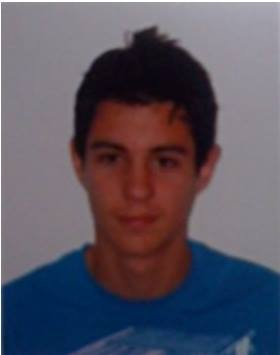
\includegraphics[scale=0.3]{000.jpg}	 
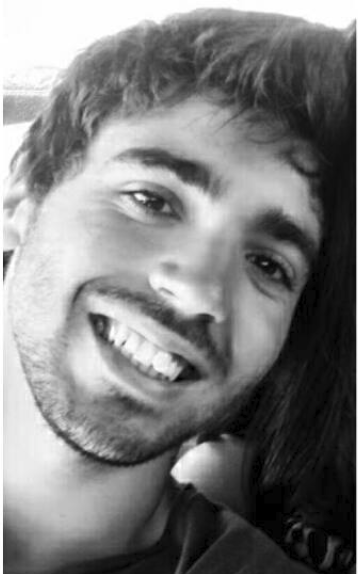
\includegraphics[scale=0.3]{001.png}
\end{figure*}


%-------------------- Inicio do Documento ----------------------------------------------------------------------



\maketitle                                            % instrução para incluir o titulo
\pagebreak
                                                        % no documento.

\section{Introdução}




%\begin{figure*}[!b]
     %   \centering
%\includegraphics[scale=0.38]{}
%\end{figure*}

\pagebreak

\section{O projeto}
\textbf{JAVA API}
\\ 
Vamos começar com a parte mais obvia de qualquer projeto.
Para conseguirmos compilar este programa, recorremos a algumas bibliotecas de JAVA, nomeadamente:

\begin{code}
java.util;
java.io;
java.text;

\end{code}


\textbf{\\ \\Imóvel}
\\

"Imóvel" é a primeira classe que começamos a fazer e é uma das duas classes do nosso programa, para conseguirmos criar imóveis mais específicos, neste caso, para dividi-los em diversas categorias para determinarmos variáveis extra. A classe é composta pelas variáveis estado, tipoImóvel, morada, precoPedido, precoMinimo e visitas. 
\\
O clone do imóvel é ligeiramente diferente dos clones de classes normais, sendo ele:
\begin{code}
...
 abstract Imovel clone();
...
\end{code}
.
\linebreak
Também temos dois tipos de toString diferentes (um para os vendedores e outro para os compradores, que mais tarde falaremos deles), para que possámos ocultar a informação do preço mínimo ao comprador.

\begin{code}
public String toString()\{
        StringBuffer s = new StringBuffer();
        s.append("\n-------------------------------\n");
        s.append(" *** "+this.tipoImovel+" ***\n ");
        s.append(" * Estado: "+this.estado+" *\n");
        s.append("Morada: "+this.morada+"\n");
        s.append("Preco Pedido: "+this.precoPedido+"\n");
        s.append("Preco Minimo: "+this.precoMinimo+"\n");
        return s.toString();
    \}
    
    public String toStringParaCompradores()\{
        StringBuffer s = new StringBuffer();
        s.append("\n-------------------------------\n");
        s.append(" *** "+this.tipoImovel+" ***\n ");
        s.append(" * Estado: "+this.estado+" *\n");
        s.append("Morada: "+this.morada+"\n");
        s.append("Preco Pedido: "+this.precoPedido+"\n");
        return s.toString();
    \}
\end{code}

\\
Também existe a opção de retornar, gravar e incrementar as visitas aos nossos imóveis para uso na classe Consulta.

\pagebreak

\textbf{"Moradia"}
\\
Esta foi a primeira subclasse que fizemos do abstract Imóvel.  
\\

\begin{code}
\end{code}


% ============================= ATÉ AQUI TUDO BEM! ========================================
\pagebreak
\textbf{Categorias}
\\
Tivemos que implementar 4 outras classes para criar um cenário de grupos de carros distintos: as categorias. 

Estas estão ligadas à classe abstrata Carro e estão também implementadas na interface Híbrido. Tem como nomes:

\begin{itemize}
\item Protótipo Classe 1
\item Protótipo Classe 2
\item Grand Turismo 
\item Stock Car
\end{itemize}

Cada categoria tem os seus construtores que geralmente usam o comando super(), o que faz com que em vez de executar os nossos métodos nas classes descendentes, subimos na herança e vamos para a nossa superclasse.

Cada classe tem a sua potência do motor híbrido definida como uma constante inalterável que irá circular com os seguintes métodos:

\begin{code}
  private int cv_h;
  
  
  public int getPotenciaMotorElectrico()\{return this.cv_h;\}
    
    public void setPotenciaMotorElectrico(int cv)\{this.cv_h=cv;\}
    
    public void inserirPotenciaHibrido()\{
        if (hibrido()==true)\{
            setCv(super.getCv() + this.cv_h);super.motor_h=1;
        \}
    \}
    
    public void removerPotenciaHibrido()\{
        if ((hibrido()==true)&&(super.motor_h==1))\{
            super.setCv(super.getCv() - this.cv_h);
            motor_h=0;
        \}
    \}

\end{code}
getPotenciaMotorElectrico() e setPotenciaMotorElectrico() são métodos get e set aparentemente normais que interagem com a variável cv\_h enquanto que os outros métodos servem para inserir e remover o motor híbrido se tiverem de ser usados para o correspondente troféu.

\pagebreak

\textbf{Híbrido}
\\
Tal como foi dito ao bocado, as classes anteriores estão ligadas a uma interface, que nos dá mais dinamismo em termos de implementar métodos, identificar facilmente objetos e de comunicação com variáveis entre classes.
Essa interface tem o nome "Híbrido" que simplesmente nos dá a possibilidade de podermos usar os métodos da potência extra do motor elétrico no nosso carro caso seja instalável e caso o campeonato tenha o troféu híbrido.

Esta classe só pode ter os enunciados dos métodos, ou seja, só pode ter uma parte dos métodos que estão definidos nas outras classes que irão ser implementadas.

\begin{code}

public boolean hibrido ();
    
public int getPotenciaMotorElectrico();
    
public void setPotenciaMotorElectrico(int cv);

\end{code}

%-------------------TUDO BEM POR AQUI ----------------------------------------------------------------------

\textbf{Equipa}

Como foi retratado em cima, para a classe Carro funcionar corretamente (visto que dentro da classe Carro temos definida uma variável do tipo Equipa) precisa também desta classe que, basicamente, serve como um elo de ligação entre os pilotos e o carro. Pela lógica, também irá precisar da classe Piloto, devido a esta receber dois pilotos para criar uma equipa e inserir num carro.

\begin{code}
private ArrayList <Piloto> equipa = new ArrayList <Piloto> (2);

...

public Piloto getPiloto1 () throws NullPointerException \{
        if (!this.equipa.isEmpty()) return this.equipa.get(0);
        else \{throw new NullPointerException ("Piloto vazio");\}
    \}

public Piloto getPiloto2 () throws NullPointerException \{
        if (this.equipa.size()<=2) return this.equipa.get(1);
        else \{throw new NullPointerException ("Piloto vazio");\}
    \}

\end{code}

Esta classe tem a curiosidade de ter gets e sets semelhantes aos que encontramos em "Carro". No entanto, a implementação da Exception faz a diferença entre elas, sendo usada por precaução, para não nos estar a aceder a memória reservada e parar o programa por completo.

\pagebreak
\textbf{Piloto}

A classe Piloto tem informações necessárias ao desenvolvimento de cada corrida que fazemos, visto que tem a qualidade geral e a qualidade com o piso normal que irão fazer muita alteração no tempo de cada volta de um circuito.

Temos uma variável provas\_v que nos dá um número de provas vencidas pelo piloto, que irá ser alterada pelo seguinte método:

\begin{code}
public void ganhouProva ()\{
        this.provas_v++;
\}
\end{code}

Basicamente, se o piloto ganhar a prova que irá fazer, incrementará o número de provas vencidas.
\\

\textbf{Circuito}

Para podermos correr com os carros numa pista, obviamente que precisamos desta classe que nos dá simplesmente as informações necessárias para que haja condições para podermos competir, como por exemplo:

\begin{itemize}
\item distancia : Vai nos dar o comprimento do circuito que irá ser usado para o cálculo do tempo da próxima volta;
\item tmv : Um HashMap que está dividido pelas categorias e tem o tempo médio de volta de cada uma;
\item n\_voltas : Número de voltas da corrida que é usado como um loop na corrida;
\item desvio\_tempo\_medio : só quando o piso estiver molhado é que esta variável atua e faz a diferença no tempo;
\item tempo\_box : que nos dá o tempo apróximado de paragem na box;
\item condicao\_piso : Se o piso está seco ou molhado.
\end{itemize}

Esta classe tem uma subclasse chamada Recorde que basicamente regista cada recorde batido por um piloto em cada pista.
\\
\\
\\

\textbf{Tempo}
\\
Esta classe tem apenas uma função: converter os segundos (Seg) da volta num formato HH:MM:SS.
É utilizado um algoritmo de divisão de segundos para converter para o que queremos.

\pagebreak

\section{Utilizador}

Quando pomos esta aplicação a correr, notámos logo de início que temos os utilizadores disponíveis para o carregamento.
\\

\textbf{Inicio}
'
\\
O início é a primeira função a ser chamada pela Main e dá-nos uma espécie de Login (o próprio método chama-se login) em que temos a opção de criar um novo perfil ou então escolher um utilizador armazenado no programa.
\\
Este método retorna-nos um inteiro muito importante para o resto do programa. Este inteiro é basicamente o número de identificação do utilizador com qual fizemos login ou do utilizador criado.
\\ 
\\
\textbf{Jogador}
\\
\\
Isto não seria possivel se não fosse esta classe que nos armazena a lista de utilizadores que ao mesmo tempo são apostadores de corridas (jogadores).
Esta classe guarda dados básicos sobre o utilizador, como o seu nome, a sua morada, o número de apostas ainda em atividade e o número de apostas ganhas.
Também temos uma espécie de conta bancária do jogador para entrar em apostas. Obviamente este valor se irá alterar conforme se ganham ou perdem apostas.

Dois métodos em destaque serão:
\begin{code} 
public int inserirAposta (String nome, String nomePista, int dinheiro, int posicao, int utilizador)\{
...

public int gerirAposta (String nome, String nomePista, int posicao)\{
...


\end{code}
que nos permitem gerir as nossas apostas que estarão armazenadas na subclasse Aposta.
\\
\\

\textbf{Aposta}

Esta classe armazena-nos toda a informação precisa para depois podermos comparar com o resultado final da prova em questão.

\pagebreak

\section{As classes ''estáticas''}

Estáticas está entre aspas porque estas classes não são propriamente estáticas. Grande parte dos métodos que estão dentro delas é que são considerados estáticos e fazem um importante papel neste programa, visto que é isto que faz executar toda a nossa atividade.
Outro fator importante destes métodos (incluindo o método login() acima referido) é, como regra de ouro: "um método não estático não pode ser referenciado a partir do contexto estático."
\\
\\

\textbf{Main}

A Main é, sem dúvidas, a maior classe do programa. Esta classe:

\begin{itemize}
\item Chama os menus que aparecerão no terminal;
\item Chama outros métodos exteriores à classe;
\item Funciona como um gigante menu gerado pelo comando switch e por um loop (usando o while);
\item Gere toda a informação de listar, editar, guardar e eliminar informação, usando outros métodos da classe;
\item Chama os métodos que carregam e guardam os nossos dados.
\end{itemize}

No entanto, vemos que a Main, em grande parte, chama os outros métodos que praticamente fazem o que ela até podia fazer, mas está dividido em diferentes classes para ordenar por contexto e para não misturar muito o código, o que faz com que mais tarde fique menos confuso a programar.

\textbf{Corrida}
\\
Esta é a classe que trata especificamente de cada prova que irá ser efetuada. Ela recebe como argumentos o campeonato que temos e um inteiro que contém o modo de como as categorias de carros irão correr.

Ela está ligada a outra classe que regista as voltas que cada carro faz numa classificação geral e numa classificação dividida por categorias. Estas classificações são ordenadas por meio de um comparator que ordena o numero de segundos de cada volta por ordem crescente.

A classe aposta vai buscar indiretamente estes valores, visto que irá ser preciso para saber se o dado utilizador ganha ou perde a sua aposta.

\begin{code}
public static void ganhaAposta(Campeonato c1)\{ 
...

\end{code}

Também temos vários métodos de controlo para gerir a probabilidade do carro ter um acidente ou de ir às boxes, com a ajuda de variáveis aleatórias.

\textbf{Campeonato}

O campeonato constrói-nos o conjunto de pistas que iremos correr, por ordem de entrada.
Também tem um método que, para entrar em funcionamento, temos de implementar a classe de sistema Serializable, para que possamos gravar o nosso campeonato.

\begin{code}
public void save(String fich) throws IOException {
        
      
      ObjectOutputStream oos = new ObjectOutputStream(
                                new FileOutputStream("Save/"+fich+".dat"));
      oos.writeObject((Campeonato) this);
      oos.flush(); oos.close();
    }
\end{code}

\section{Outras classes}
  
\textbf{Titulos}

Titulos é basicamente a classe que é chamada por todas as classes que queiram mostrar indicações ao utilizador. No caso do método main\_Menu2, ele mostra-nos o que temos de escrever para inserir um piloto, ou para listar todas as apostas que o utilizador fez, entre outros processos.
\\
\\

\textbf{Info\\}
Esta classe recebe informação de outra classe que se designa por Info. Isto foi uma maneira de representar os movimentos mais importantes que nós fazemos no próprio menu de títulos.  
\\

\textbf{CCInvalidaException\\}
CCInvalidaException é usada especialmente quando queremos criar um carro de uma dada categoria. Como as categorias têm limites no que toca às cilindradas dos carros, se inserirmos uma cilindrada inválida, o programa não será interrompido com uma exceção de sistema.
\\


%-------------------- ISTO É UM SEPARADOR ... A SÉRIO----------------------------------------------------------------------
 
\section{Conclusão}
Este projeto deu muito trabalho em relação aos ficheiros. Posso dizer que tive extrema dificuldade em gravar e carregar jogos devido à particularidade de ter de gravar as variáveis uma a uma e não um ''campeonato''  inteiro.

Falando um bocado sobre a suposta ''regra de ouro'' que tratei em cima ''um método não estático não pode ser referenciado a partir do contexto estático'' por curiosidade esta também foi outra das minhas dificuldades. Na altura fiquei muito confuso e frustado por não poder misturar estes dois conceitos, visto estar habituado à linguagem C, onde não havia limitações nesse aspeto.

Uma das estruturas que mais devo ter utilizado neste projeto e que me deu imenso jeito é o Random Int, para poder calcular as probabilidades dos carros terem acidentes ou terem ido à boxe, entre outros.

Este trabalho foi extremamente produtivo e só me trouxe vantagens para conhecer o mundo dos objetos.

\end{document}